\documentclass[11pt]{article}
\usepackage{../EllioStyle}
\usepackage{listings}

\definecolor{codegreen}{rgb}{0,0.6,0}
\definecolor{codegray}{rgb}{0.5,0.5,0.5}
\definecolor{codepurple}{rgb}{0.58,0,0.82}
\definecolor{backcolour}{rgb}{0.95,0.95,0.92}

\lstdefinestyle{mystyle}{
%    backgroundcolor=\color{backcolour},   
    commentstyle=\color{codegreen},
    keywordstyle=\color{magenta},
    numberstyle=\tiny\color{codegray},
    stringstyle=\color{codepurple},
    basicstyle=\ttfamily\footnotesize,
    breakatwhitespace=false,         
    breaklines=true,                 
    captionpos=b,                    
    keepspaces=true,                 
    numbers=left,                    
    numbersep=5pt,                  
    showspaces=false,                
    showstringspaces=false,
    showtabs=false,                  
    tabsize=2
}

\title{Homework 2}
\author{Elliott Pryor}
\date{7 September 2021}

\rhead{Homework 2}

\begin{document}
\maketitle

\problem{1}

Propose a dynamic programming algorithm to solve longest common substring problem
\hrule

This is almost identical to the Edit Distance algorithm.

We create $V = nxm$ matrix. We set $V_{0,0} = 0$, and $V_{i,0} = 0, V_{0,j} = 0$ because the longest common subsequence
is at least 0 (by matching no characters together).

We then let $V_{i,j} = \begin{cases}
    V_{i-1, j-1} + 1 & \text{if } S[i] = T[j]\\
    \max(V_{i, j-1}, V_{i-1, j}) & \text{otherwise}
\end{cases}$ for $i,j \neq 0$.
The first case handles a match between two characters.
The second case skips a character (because subsequence can be non-consecutive).

The length of the longest common substring is $V_{n,m}$.

We can also construct the alignment of the common subsequence in the same way as in Needleman-Wunch.


\begin{proof}
    Correctness.
    
    By induction, we show that $V_{i,j}$ is LCS (longest common substring) of $S[1..i]$ and $T[1..j]$.
    For $i, j = 0$ this is trivially true by matching empty strings.
    
    % Assume that $S[i] = T[j]$. Then the characters match. So the length of the LCS is $1 + $ previous length.
    % By inductive assumption we assume that $V_{i-1, j-1}$ is the LCS for $S[1 .. i-1]$, $T[1 .. j-1]$.
    % Then we can match one more character. $V_{i,j} = 1 + V_{i-1, j-1}$.
    
    % Then assume that $S[i] \neq T[j]$. 
    We assume that $V_{i-1, j-1}, V_{i, j-1}, V_{i-1, j}$ are the LCS for their respective substrings.
    Suppose $V_{i,j}$ is not the length of longest common subsequence.
    Assume $S[i] = T[j]$. Then $V_{i,j} = 1 +  V_{i-1, j-1}$. 
    Then, either we shouldn't match $S[i], T[j]$ which we can get a longer LCS at no consequence by matching them.
    Or $V_{i-1, j-1}$ is not an LCS. A contradiction in both cases.

    Then assume $S[i] \neq T[j]$. If we match against $V_{i-1, j-1}$ we break the substring since they don't match.
    So we want to skip one letter of the string. If we skip a letter in $S$ then we choose $V_{i-1, j}$.
    Suppose there is a more optimal choice. Then, we shouldn't have skipped a letter in S (and instead in T), which is handled
    by the other case of the $\max$. Or $V_{i-1, j}$ is not optimal, which is a contradiction.
    The same holds in reverse for choosing to skip a letter in T. 

    Thus inductive step holds by contradiction in all cases.

\end{proof}


\problem{2}
Given two sequences S, T (not necessarily the same length), let G, L, H be the scores of the
optimal global alignment, optimal local alignment, and optimal global alignment without penalizing leading or trailing spaces.


\begin{enumerate}[a)]
    \item Give an example of S, T so that the three scores are different
    \item Prove or disprove the statement $L \geq H \geq G$
\end{enumerate}

\hrule

\begin{enumerate}[a)]
    \item S = aaatata, T = tatc
    G = 2, L = 6, H = 5

    \item It is correct.
    \begin{proof}
        We first prove $L \geq H$ by contradiction.
        Suppose not, then $L < H$. 
        Given some global alignment $S, T = H$ (S, T) are globally aligned strings. 
        Let $a$ be the first non-space character in $T$, and $b$ be the last non-space character in $T$.
        Similarly, let $c$ be the first non-space character in $S$, and $d$ be the last non-space character in $S$.
        Then construct substrings $S' = S[a .. b], T' = T[c .. d]$.
        Then the alignment of $S', T' = H$. Since leading and trailing spaces
        are not penalized in $H$, $S', T'$  consist of only the characters that are scored in $H$.
        Since $S', T'$ are valid substrings, we have a contradiction. 

        Now we prove $H \geq G$ by contradiction.
        We assume that $H < G$. Since $G$ is the optimal global alignment.
        We can choose an alignment for H to be the same as this global alignment. 
        Then clearly $H \geq G$, since if $G$ has no leading or trailing spaces $H = G$.
        Thus a contradiction.

        Therefore $L \geq H \geq G$
    \end{proof}

\end{enumerate}


\problem{3}

Implement the global alignment algorithm from class.  Your program should read in a FASTA file (see HW1).  You can assume that the file just contains two sequences, e.g.

$>$ seq1\\
ACTGGGAAA\\
$>$ seq2\\
CTGGAACA

The filename should be supplied as a command-line parameter.

Align the first string with the second string.  Print out one optimal alignment.

You can assume a simplified scoring function delta that has the following form:
delta(match) = 2
delta(mismatch) = -1
delta(insertion/deletion) = -1

Demonstrate your algorithms on two test cases (use screen shots to show runs). 

\hrule

\begin{figure}[h]
    \centering
    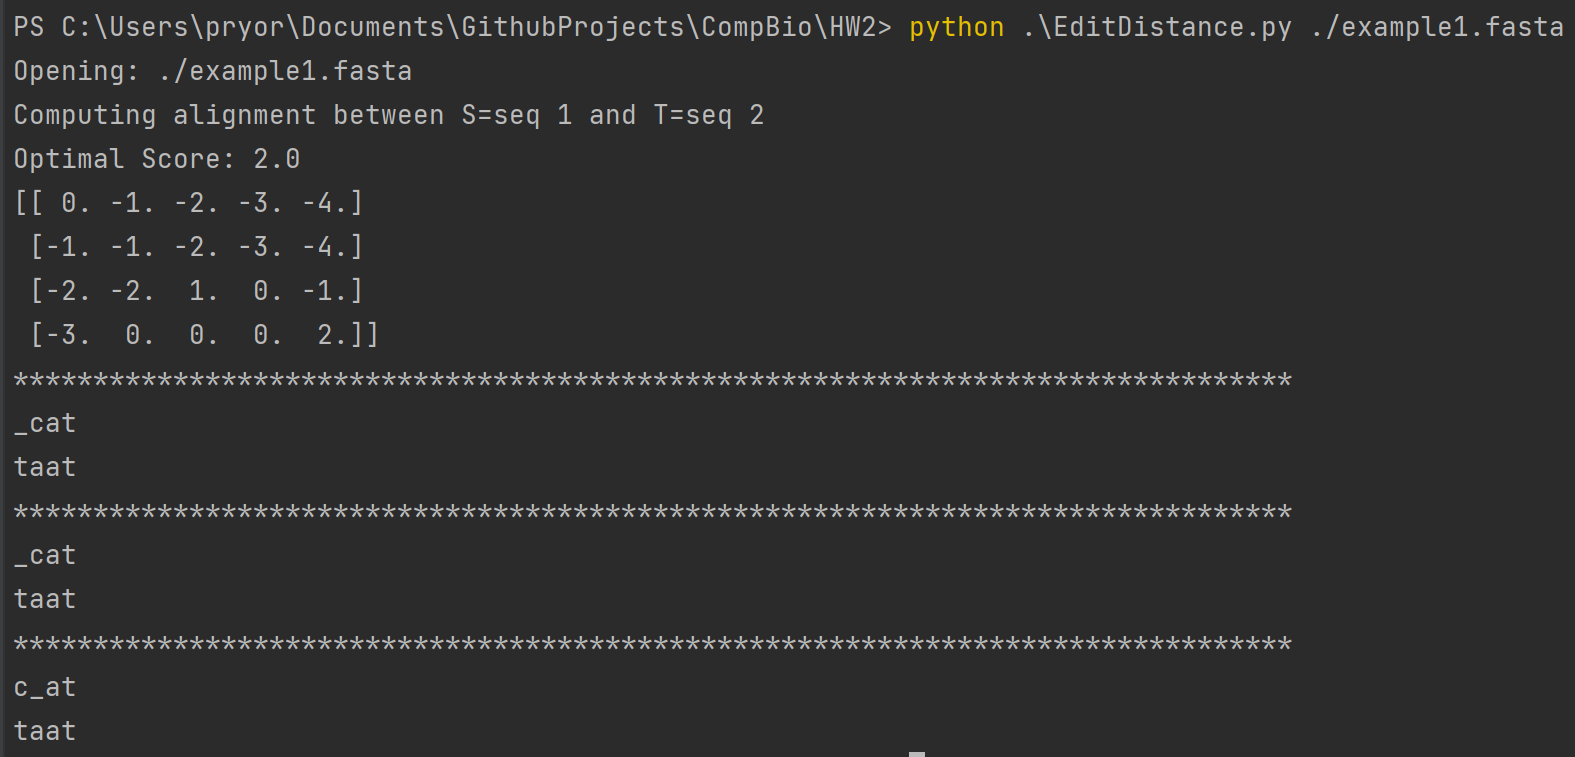
\includegraphics[width=0.55 \linewidth]{./example1.png}
    \label{fig1}
    \caption{Example 1, using cat and taat from class}
\end{figure}

\begin{figure}[h]
    \centering
    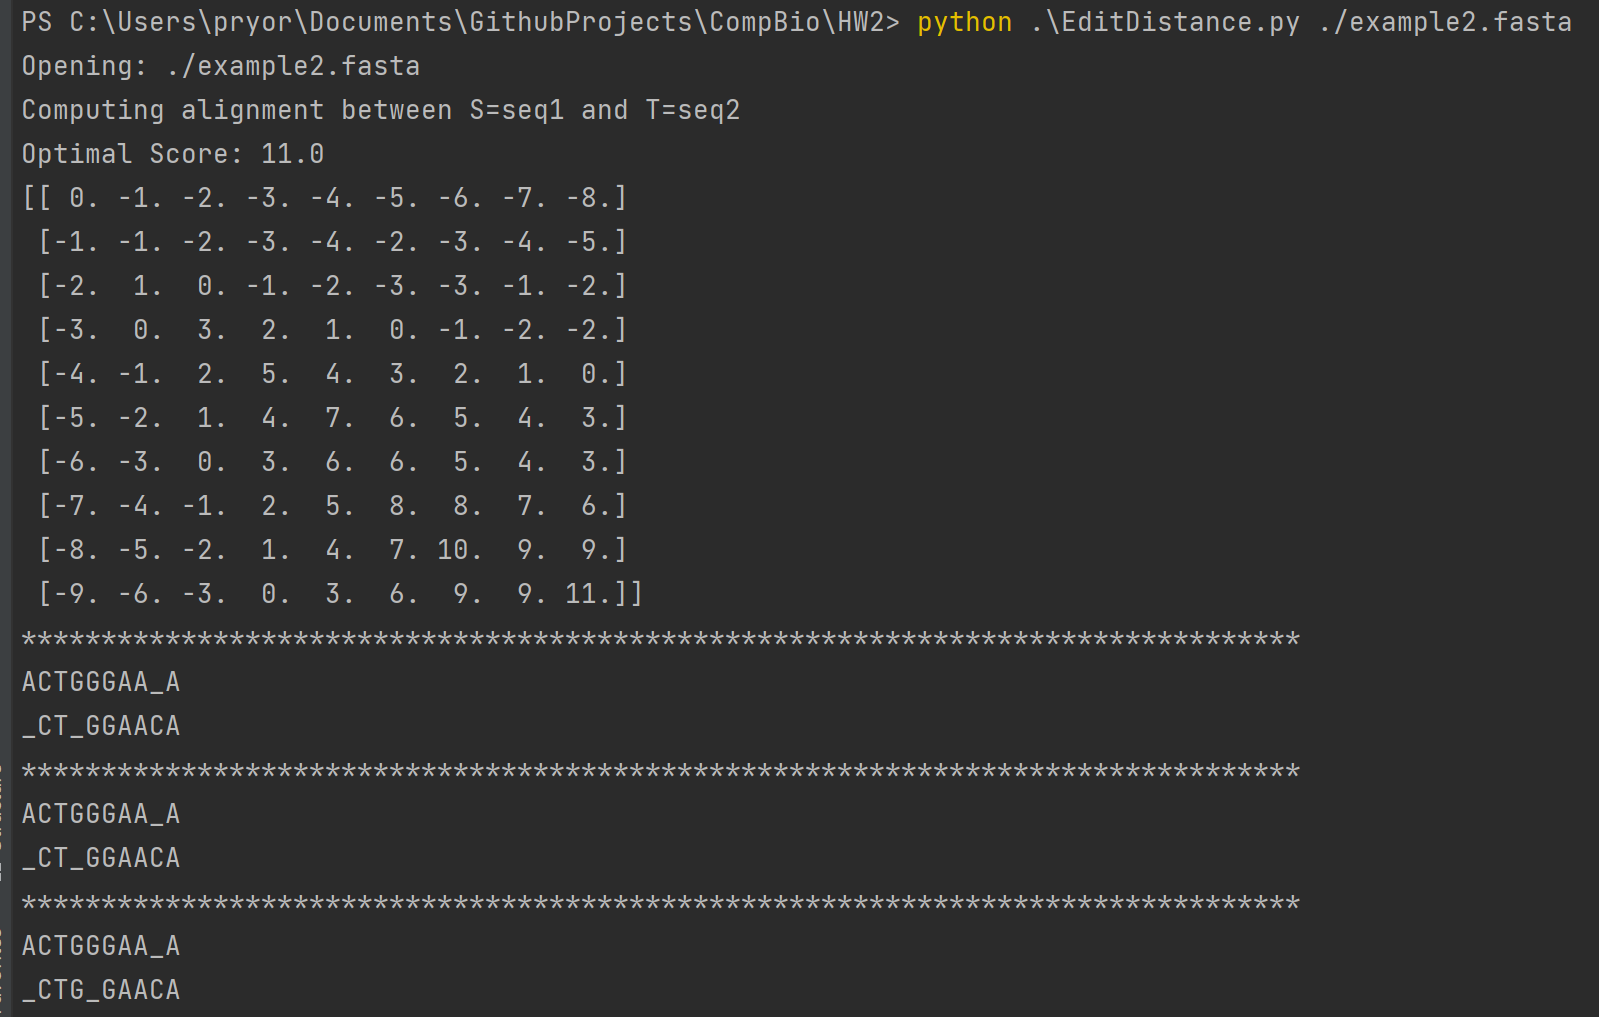
\includegraphics[width=0.55 \linewidth]{./example2.png}
    \label{fig2}
    \caption{Example 2, using input from the homework description}
\end{figure}

I did the bonus and we can see that it prints all optimal alignments. 
It produces duplicated results because I don't use a set,
and the first move can take 2 paths and produce the same path.
Consider example 1 from class. We can go (0,0) $\rightarrow$ (0,1) $\rightarrow$ (2,1)
or (0,0) $\rightarrow$ (1,1) $\rightarrow$ (2,1). Both just add a space to the front of cat.
So they are indeed 2 different paths with the same `phenotype'. 

\lstset{style=mystyle}
\lstinputlisting[language=Python]{EditDistance.py}


\end{document}